{\Large Architectural Design patterns} \\\\
 VR presentation Valknut Software Engineering \\\\
During the process of creating a 3D environment we have employed the effectiveness of certain design patterns to help simplify the interaction between the user and the environment itself. The architectural patterns we have used are as follows:\\\\
1.	Factory Design Pattern\\
2.	Memento Design Pattern\\
3.	Prototype Design Pattern\\\\
	\section{Justification of Design pattern use:}
	\subsection{Factory}
	In the VR presentation software we have created an interface whereby the players/users are able to create and instantiate 3D objects. This creation is facilitated through our use of a factory design method. By providing the interface for the user to create these 3D objects they can then make use of a set of subclasses to determine the specifics of what objects is to be made.\\\\
	\subsection{Memento}
	We plan to utilize the memento design pattern in a manner that is seen across many different gaming environments. Due to users being able to create customized worlds and environments it became an imperative that they are able to save their work. The ability to capture the game environments internal state and then recall that from storage will be executed with the Memento design pattern to allow restoration to a specific point.\\\\
	\subsection{Prototype}
	In the 3D environment one of the essential functions was that after a user had finished scaling and rotation an object they should be able to create a duplicate of this object, using the pre-existing object as some form of prototype. This meant that through implementing the Prototype design pattern we were able to create a platform where they could achieve this cloning functionality.
  	\subsection{Actvity Diagram}
	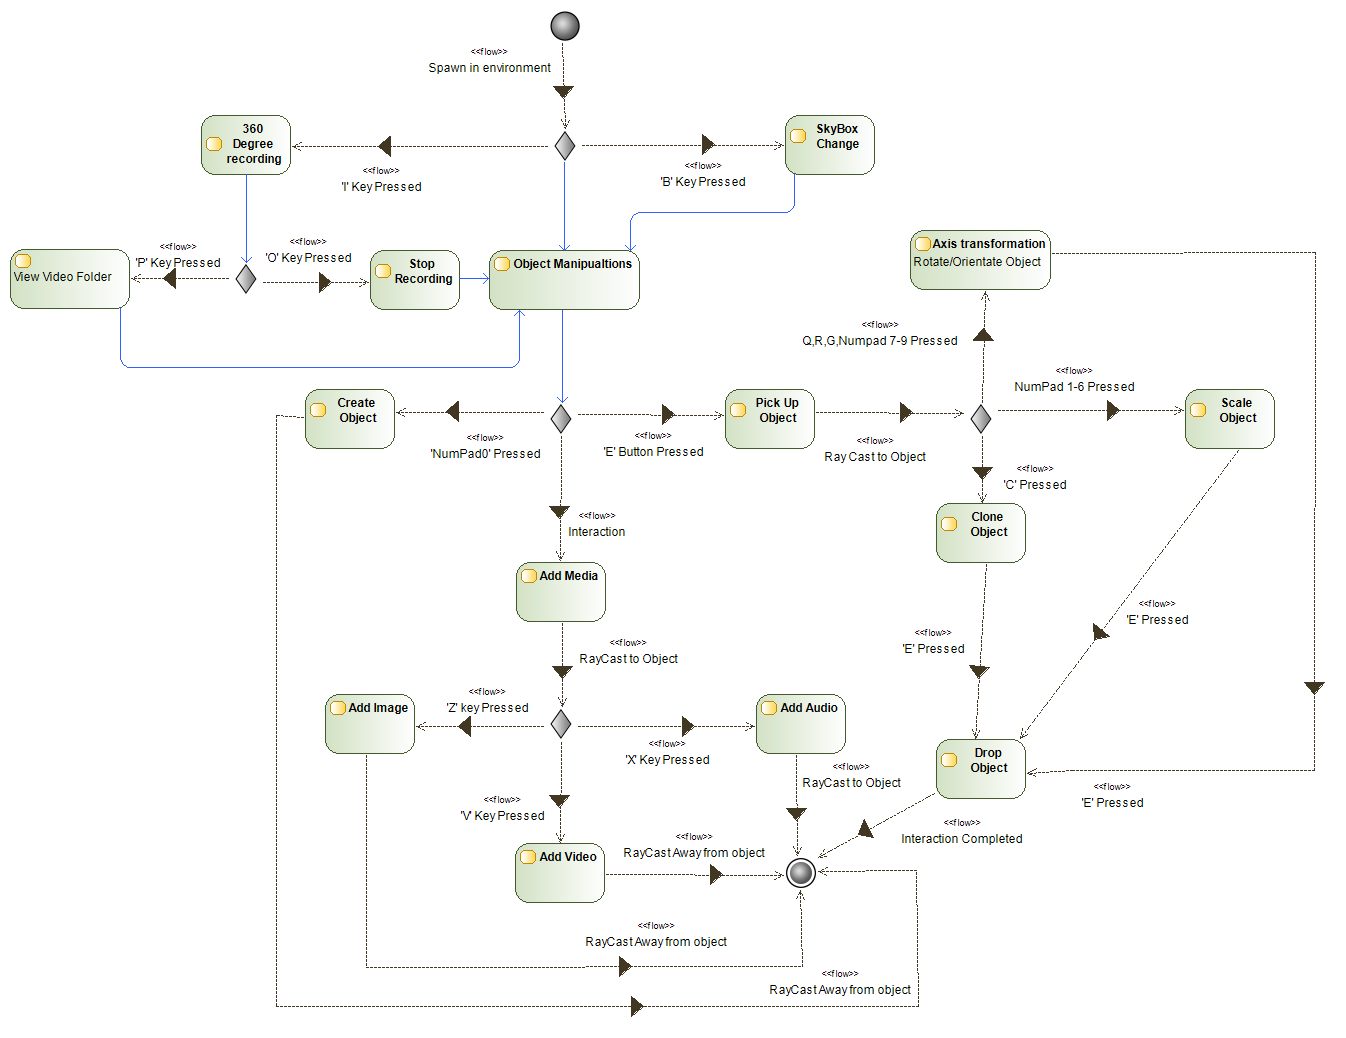
\includegraphics[width=450px,height=325px]{ActivityDiagram.png}

	\section{Deployment Diagram:}
	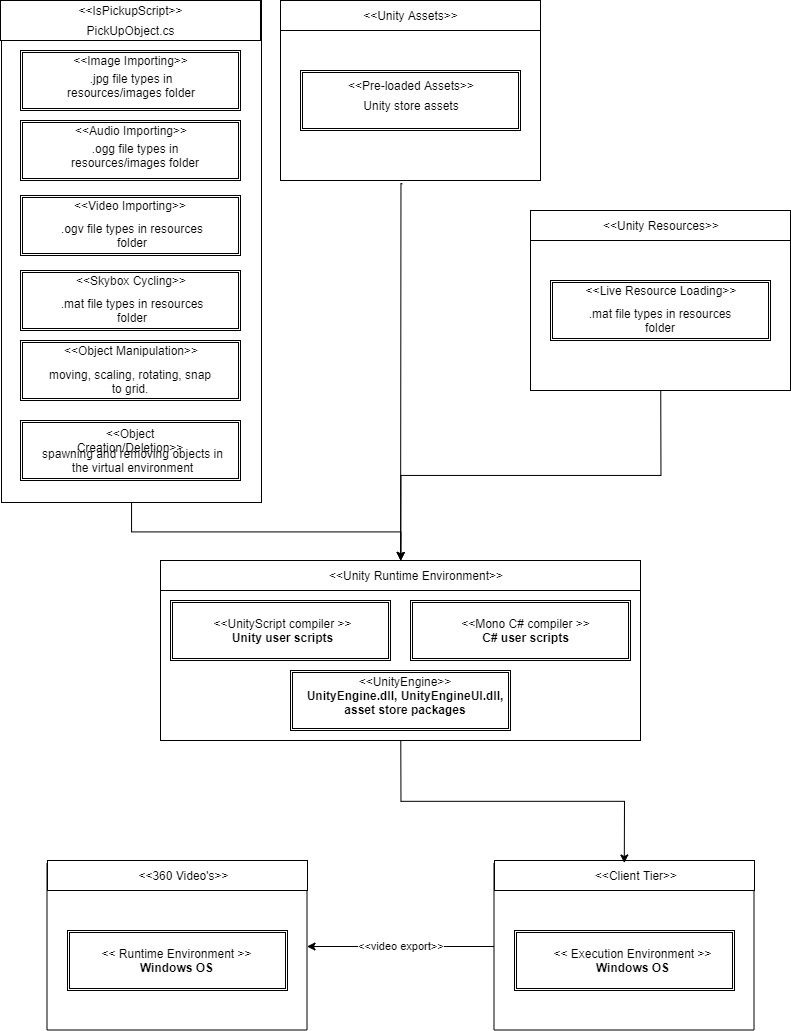
\includegraphics[width=450px,height=550px]{DeploymentDiagram.png}
